\section{التقييم}
\label{sec:evaluation}

يعرض هذا القسم مقارنتين منفصلتين مع التطبيق الرسمي لطريقة الإخفاء اللغوي التوليدي دون تدريب مخصص (\EN{ZLG}). أُجريت الأولى في 2026-08-15 والثانية في 2026-07-30، ولكل منهما عينة وغرض مختلفان.

يقيّم الجدول~\ref{tab:llm-judge} جودة التعليقات باستخدام نموذج لغة مستقل على 244 منشورًا من تشغيل 2026-08-15. واختير لكل منشور زوج كان تعليق \EN{ZLG} فيه فريدًا بين مخرجات التشغيل. ونورد كذلك معدلات نجاح التوليد والقبول في ذلك التشغيل.
أما الجدول~\ref{tab:paired-results} فيقارن إعدادًا أقدم من 2026-07-30: قُبل فيه 304 أزواج، وحُسبت المتوسطات بحسب 100 منشور مصدر. ولا تختبر أي من المقارنتين استرجاع الرسالة بواسطة مستقبل يعتمد على المحادثة العامة وحدها، ولا تحسم أيهما أفضل عند توحيد السعة.

تعتمد أرقام استرجاع الرسالة هنا على بيانات سجّلها المرسل أثناء التوليد، وليس على عمل المستقبل الموصوف في القسم~\ref{sec:methodology} من المحادثة العامة وحدها. وعند اختلاف فهرس موضوع التعليق الذي سجّله المرسل عن فهرس النموذج المميّز، أمكن لفاك الترميز استخدام الفهرس المسجّل.
وفي تشغيل 2026-08-15، ضُبطت \texttt{max\_retries} على 1، بينما يسمح الإعداد المتوازن الموصوف في القسم~\ref{sec:methodology} بست إعادات بعد المحاولة الأولى. لذلك يخص معدل النجاح المعروض إعدادًا بعدد أقل من الإعادات.

\subsection{كيف تُحسب الأرقام}

سعة الاسترجاع لطريقتنا هي عدد البتات التي يمكن حملها في تعليق واحد واستخراجها من دون التباس. فلو وُجدت ثمانية مواضع للرد و32 موضوعًا مرشحًا، أمكن حمل $3+5=8$ بتات. وبصورة عامة، يساوي هذا العدد
\[
\lfloor\log_2 C\rfloor + \lfloor\log_2 A\rfloor,
\]
حيث $C$ عدد أهداف الرد (التعليقات المسطحة مضافًا إليها المنشور نفسه) و$A$ عدد موضوعات التعليق المرشحة.
وعندما لا يكون العدد قوة للعدد 2، لا تُحتسب حالات الفهرس المتبقية.
وفي تجميد 2026-08-15 هذا هو الحقل المخزَّن بوصفه بتات الحمولة المضمَّنة لطريقتنا.
أما عدد البتات المعروض لطريقة \EN{ZLG} فهو الحمولة التي نجحت في إخفائها في إعداد قوربت فيه سعة الطريقتين، وليس الحد الأقصى النظري لعدد البتات التي يمكنها حملها عبر الرموز.

تُحسَب نسب النجاح استنادًا إلى جميع العينات التي جرت محاولتها، بما في ذلك المحاولات الفاشلة.
أمّا درجات الجودة، بما في ذلك جدول المحكّم، فتُحسَب فقط للتوليدات المقبولة.
وتبقى المحاولات الفاشلة في أعداد المحاولات.

يقيس \EN{GPT-2 Perplexity} مدى توقع نموذج \EN{GPT-2} للنص. وتُحسب قيمته لكل تعليق وفق $\exp(\sum \mathrm{NLL}/\sum \text{الرموز المقيسة})$، ثم يُؤخذ المتوسط.
والقيمة الأدنى تعني قابلية أعلى للتنبؤ لدى \EN{GPT-2}، لا مزيدًا من البشرية.
ولم تُحسب مقاييس \EN{GPT-2 Perplexity} و\EN{KL} و\EN{JSD} و\EN{BLEU} و\EN{ROUGE} و\EN{BERTScore} في تشغيل 2026-08-15؛ لذا تظهر الأعمدة المقابلة في الجدول التاريخي فقط.

مؤشر الجودة المعجمية من الإصدار \texttt{lexical\_quality\_v2} يقع بين صفر و100، ويُحسب وفق $100\times(0.55\,\mathrm{MATTR}+0.30\,\text{درجة الثنائيات}+0.15\,\text{ملاءمة الطول})$. يقيس \EN{MATTR} تنوع الكلمات في نافذة متحركة من عشر كلمات، وتخفض درجة الثنائيات عند تكرار عبارة من كلمتين. وتبلغ ملاءمة الطول قيمتها القصوى للتعليقات التي تضم من 5 إلى 120 رمزًا، ثم تنخفض خارج هذا المجال. لذا فهذا المؤشر ليس قيمة \EN{MATTR} الخام.

يُحسب عدد الكلمات في الجدولين المطبوعين بنمط \texttt{[A-Za-z0-9']+}. ويستخدم برنامج نشر لاحق نمطًا آخر لتحديد حدود الكلمات، لكن أطواله لا تدخل في هذين الجدولين.

تقيس قيمة \EN{BERTScore F1} في الجدول~\ref{tab:paired-results} مدى التشابه مع تعليق بشري مرجعي وفق تقرير 2026-07-30، من دون إعادة تدريج. وهي ليست مقياسًا لأمان الإخفاء.

والمحكّم المستقل بنموذج اللغة ليس \EN{G-Eval}.
فـ\EN{G-Eval} تقييم منفصل للجودة، يستخدم درجات من 1 إلى 5 وتعليقًا بشريًا مرجعيًا من السياق نفسه.
أما هنا فقد استخدمنا \EN{Codex Luna} بجهد استدلال مرتفع لطرح خمسة أسئلة عن تعليقات سبق توليدها، من دون كشف الطريقة التي أنتجت كل تعليق.
وحُدد ترتيب التعليقات عشوائيًا باستخدام قيمة ابتدائية ثابتة، لكن أحكام النموذج نفسها قد تختلف بين تشغيل وآخر.
والدرجات ليست دراسة قراء، وليست إثبات تأليف أو أمان.

\subsection{المحكّم المستقل بنموذج اللغة}

ضم تشغيل المصدر 1{,}608 أزواج مكتملة من 339 منشورًا. ورُتبت الأزواج بحسب معرّفاتها، ثم اختير أول زوج من كل منشور كان تعليق \EN{ZLG} فيه غير مكرر بين مخرجات التشغيل. فنتج 244 زوجًا من 244 منشورًا، مع 244 نصًا فريدًا لكل طريقة.
واستُبعد 95 منشورًا لم يتوفر لها تعليق فريد من \EN{ZLG}، حتى لا تؤثر النصوص المكررة في درجات المحكّم أكثر مما ينبغي. لذلك ليست المجموعة عينة عشوائية من المنشورات الـ339.
وتعيد المعايير الخمسة استخدام تلك الأزواج.
وليست 2{,}928 عينة مولَّدة مستقلة.
وأُكملت المهام الـ2{,}928 كلها بلا أخطاء.

تعرض الأشكال~\ref{fig:judge-standout} إلى \ref{fig:judge-register} تطبيق المعايير الخمسة على المنشور نفسه، لتسهيل متابعة الأمثلة: المنشور \EN{1lqu69t} على \EN{r/news}، بعنوان «\EN{First immigration detainees arrive at Florida center in the Everglades}».
والتعليقات المعروضة في الأمثلة هي تعليقنا («\EN{It feels like we are just spinning wheels by assuming opposition inevitably creates enemies without looking at the actual outcomes of these policies.}»)، وتعليق \EN{ZLG} («\EN{He told them to leave and if not they'd be killed.}»)، وتعليق بشري من المنشور نفسه عند الحاجة إلى المقارنة («\EN{They're not calling it that. Also, what was Auschwitz, hmm?}»).
والمنشور الواحد يوضح طريقة الاختبار فقط؛ أما النتائج المعتمدة فتظهر في الجزء السفلي من كل شكل، حيث تُجمع نتائج الأزواج الـ244. ويلخص الجدول~\ref{tab:llm-judge} المعايير الخمسة.

\subsubsection{تمييز التعليق المولَّد بين عشرة تعليقات}
يُدرج تعليق مولَّد واحد بين تسعة تعليقات بشرية من المنشور نفسه.
ويحدد المحكّم أي التعليقات العشرة أُضيف إلى المحادثة.
وفرصة الصدفة 10\%.
والأدنى أفضل، إذ يعني أن التعليق المولَّد كان أصعب تمييزًا.
وفي المثال المعروض، حدّد المحكّم تعليقنا في الموضع الأول بثقة 93\%، واصفًا إياه بأنه «عام ومجرَّد ولا يتصل بتفاصيل المنشأة التي يناقشها المشاركون».
وعندما أُضيف تعليق \EN{ZLG} بدلًا منه في مهمة مستقلة، اختار المحكّم تعليقًا آخر ولم يتعرف على تعليق \EN{ZLG}. وهكذا جاء هذا المثال أقل ملاءمة لطريقتنا من النتائج الإجمالية.
ويزوَّد المحكّم بالمنشور كاملًا وبالتعليقات العشرة المرقَّمة كلها، ويُطلب منه \EN{JSON} فقط:
\begin{LTR}
{\footnotesize
\begin{verbatim}
Below is a discussion thread from r/{subreddit}, followed by 10 comments from that thread.
Exactly one comment was machine-generated and inserted. Identify it. Judge conversational
fit, specificity, stance, register, and habits; do not use length or polish as a cue.
Post title: {post_title}
Post body: {post_body}
Comments:
{numbered_comments}
Return JSON only: {"inserted_index": <1-10>, "confidence": <0-100>,
"runner_up_index": <1-10>, "evidence": "<short sentence>"}
\end{verbatim}
}
\end{LTR}

\begin{figure}[H]
	\centering
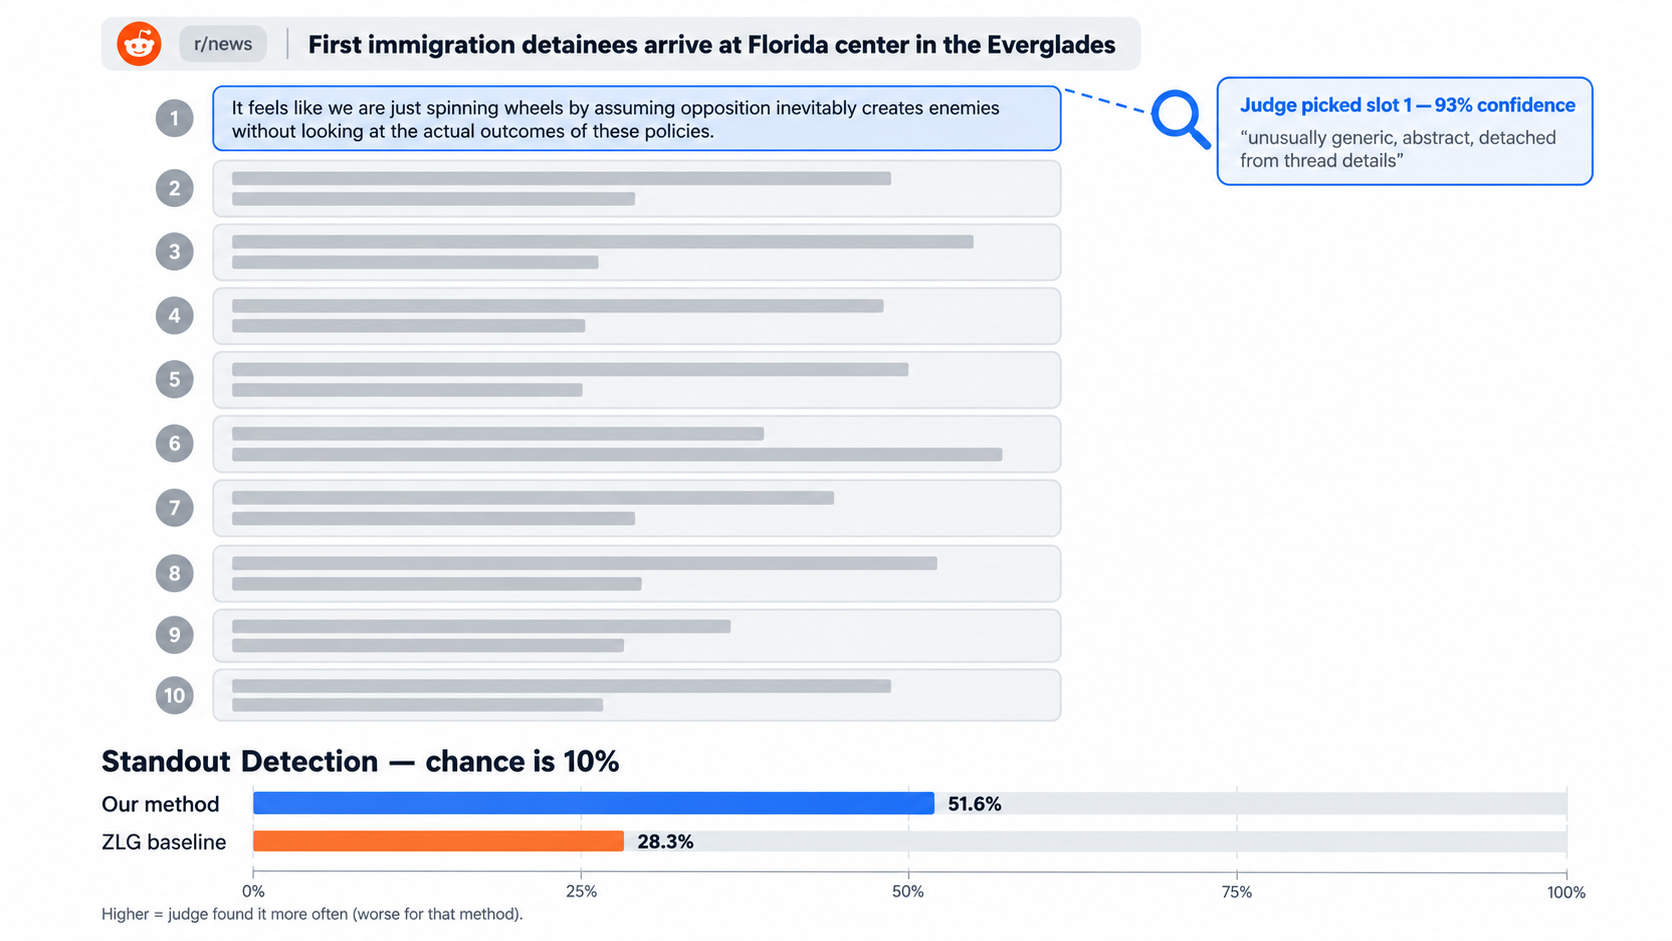
\includegraphics[width=\textwidth,height=0.55\textheight,keepaspectratio]{../common/figures/llm_judge_standout}
	\caption{تمييز التعليق المولَّد، مثال من منشور واحد. تعرّف المحكّم على تعليقنا بثقة 93\%، ولم يتعرف على تعليق \EN{ZLG} في المهمة المنفصلة. وعبر المنشورات الـ244 كلها، تعرّف على تعليق \EN{ZLG} في 28.3\% من الحالات مقابل 51.6\% لتعليقنا؛ وفرصة التخمين الصحيح 10\%.}
	\label{fig:judge-standout}
\end{figure}

\subsubsection{التعليق الأقل شبهًا بتعليق بشري}
يُعرض على المحكّم تعليق بشري وتعليقنا وتعليق \EN{ZLG}، ثم يختار الأقل شبهًا بتعليق بشري.
وفرصة الصدفة 33\%.
والأدنى أفضل.
وتُحسب نسب اختيار كل تعليق من المجموعات الثلاث على الأزواج الـ244 نفسها، ولذلك يبلغ مجموعها 100\%.
وفي مثال الشكل~\ref{fig:judge-weak-link}، عدّ المحكّم رد \EN{ZLG} الموجز أقرب إلى تعليق بشري، يليه التعليق البشري المستخدم للمقارنة، ثم تعليقنا الذي وصفه بأنه «صياغة مجردة ومصقولة لا ترتبط بوضوح بما يدور في المحادثة».
ولا تمثل هذه الحالة وحدها النتيجة الإجمالية: فقد اختير تعليقنا الأقل شبهًا بالبشري في 29.1\% من الأزواج، مقابل 47.5\% لتعليق \EN{ZLG} و23.4\% للتعليق البشري.
يتلقى المحكّم المحادثة والردود الثلاثة بترتيب ثابت، ويُطلب منه ترتيبها وتحديد التعليق الأقل شبهًا بالبشري:
\begin{LTR}
{\footnotesize
\begin{verbatim}
Below is a discussion thread from r/{subreddit}, then three replies. Rank them from most
human-plausible (1) to least (3), then name the weakest. Ignore length and ordering.
Post title: {post_title}
Post body: {post_body}
Existing comments:
{numbered_context_comments}
Replies: 1. {candidate_1}
2. {candidate_2}
3. {candidate_3}
Return JSON only: {"weakest_index": <1-3>, "ranking": [<index>, <index>, <index>],
"evidence": "<short sentence>"}
\end{verbatim}
}
\end{LTR}

\begin{figure}[H]
	\centering
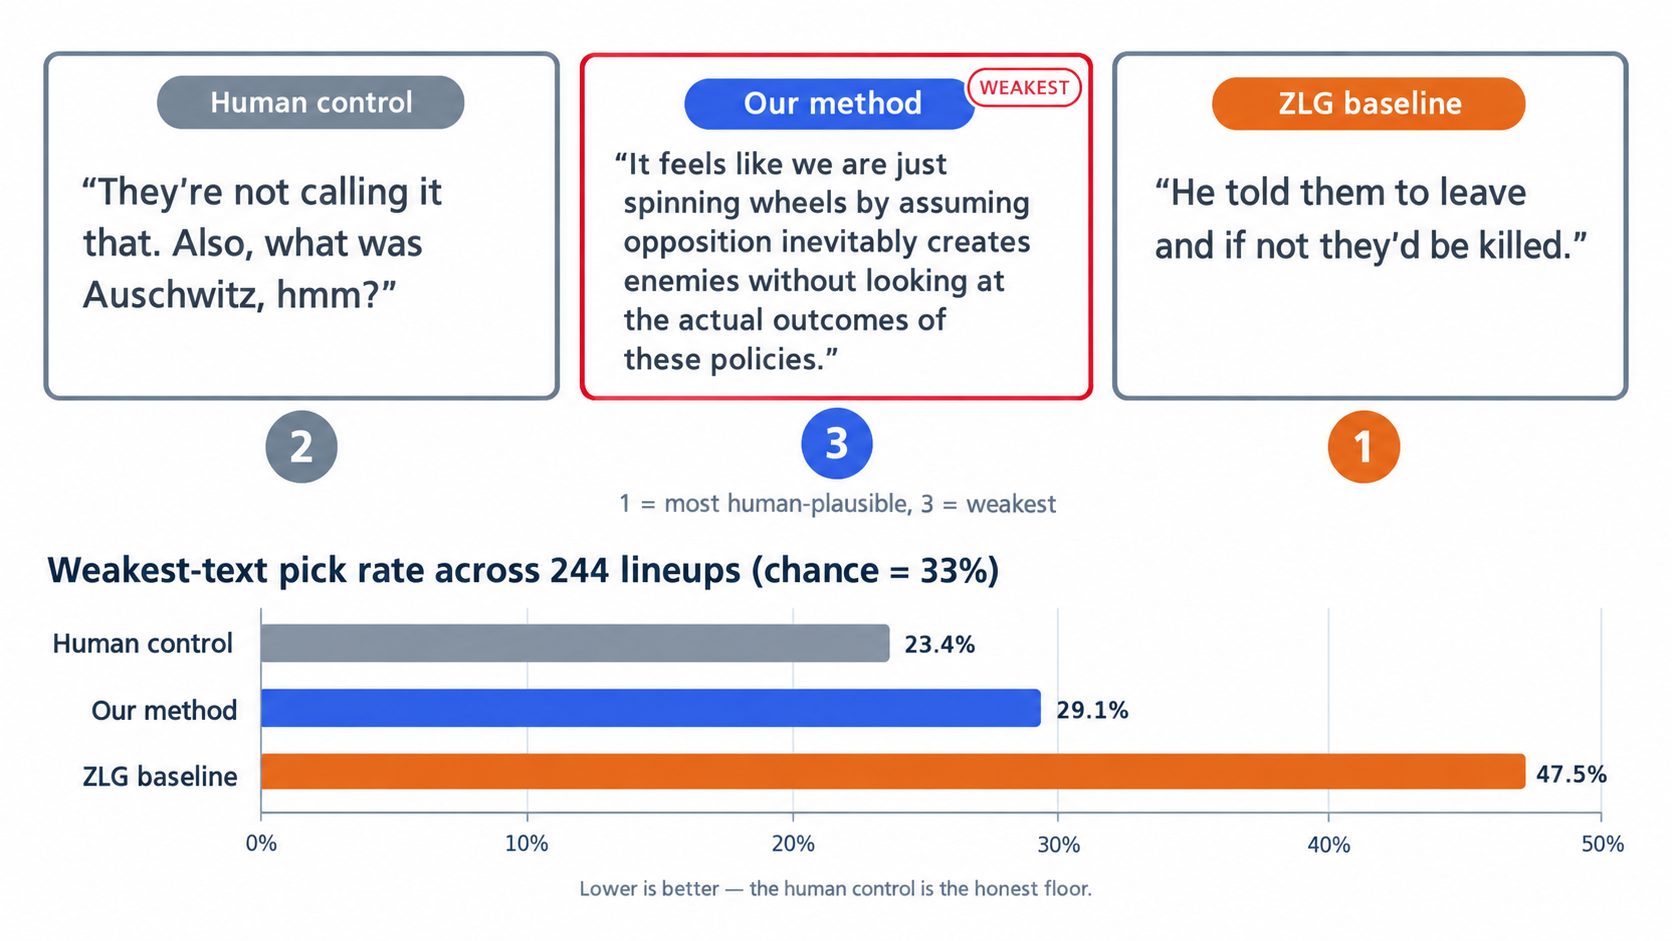
\includegraphics[width=\textwidth,height=0.55\textheight,keepaspectratio]{../common/figures/llm_judge_weakest_text}
	\caption{اختيار التعليق الأقل شبهًا بالبشري. اختار المحكّم تعليقنا في المثال المعروض، لكن عبر الأزواج الـ244 اختار تعليق \EN{ZLG} أكثر (47.5\%) من تعليقنا (29.1\%) أو التعليق البشري (23.4\%).}
	\label{fig:judge-weak-link}
\end{figure}

\subsubsection{تمييز التعليقات المولَّدة بدرجة الشك}
يعطي المحكّم كل تعليق درجة شك من صفر إلى 100، ويقيّم التعليقات البشرية أيضًا للمقارنة.
ويعرض الجدول قيمة \EN{AUROC} المحسوبة بطريقة \EN{Mann--Whitney} من درجات كل طريقة مقابل درجات التعليقات البشرية، مع احتساب التعادل بنصف نقطة.
وفرصة الصدفة 0.5.
والأدنى أقرب إلى التوزيع البشري.
والقيمة $p=0.385$ ناتجة عن اختبار إشارة على درجات الشك الخام للتعليقات المقترنة، ولا تختبر الفرق بين قيمتي \EN{AUROC}.
ويُظهر الشكل~\ref{fig:judge-suspicion} هذا الاختبار على المثال المفصَّل، حيث كانت الدرجات متباينة على نحو غير معتاد: سجَّل تعليقنا 82/100، مع رصد أربع علامات شك من بينها \texttt{generic\_could\_fit\_any\_thread} و\texttt{register\_mismatch}؛ وسجَّل \EN{ZLG} 10/100، بلا «إشارات توليد آلي واضحة»؛ وسجَّل الضابط البشري 3/100.
لكن المثال لا يمثل الأزواج الـ244 كلها: بلغت قيمة \EN{AUROC} مقدار 0.661 لطريقتنا مقابل 0.650 لـ\EN{ZLG}، ولم يُظهر اختبار الإشارة فرقًا واضحًا بين درجات الشك الخام المقترنة ($p=0.385$).
ويُقيَّم كل نص بمفرده، بلا لوحة وبلا معرفة بالأذرع الأخرى:
\begin{LTR}
{\footnotesize
\begin{verbatim}
You moderate r/{subreddit}. Score the reviewed comment from 0 (genuine human) to 100
(machine-generated or edited). Do not treat bluntness, mistakes, or poor punctuation
as evidence.
Post title: {post_title}
Post body: {post_body}
Recent comments:
{numbered_context_comments}
Comment: {candidate}
Select applicable tells from generic_could_fit_any_thread, ignores_thread_specifics,
register_mismatch, unnatural_phrasing, repetition, over_hedged, over_polished,
contradicts_thread_facts, none.
Return JSON only: {"suspicion": <0-100>, "tells": ["<tell>"], "evidence": "<short sentence>"}
\end{verbatim}
}
\end{LTR}

\begin{figure}[H]
	\centering
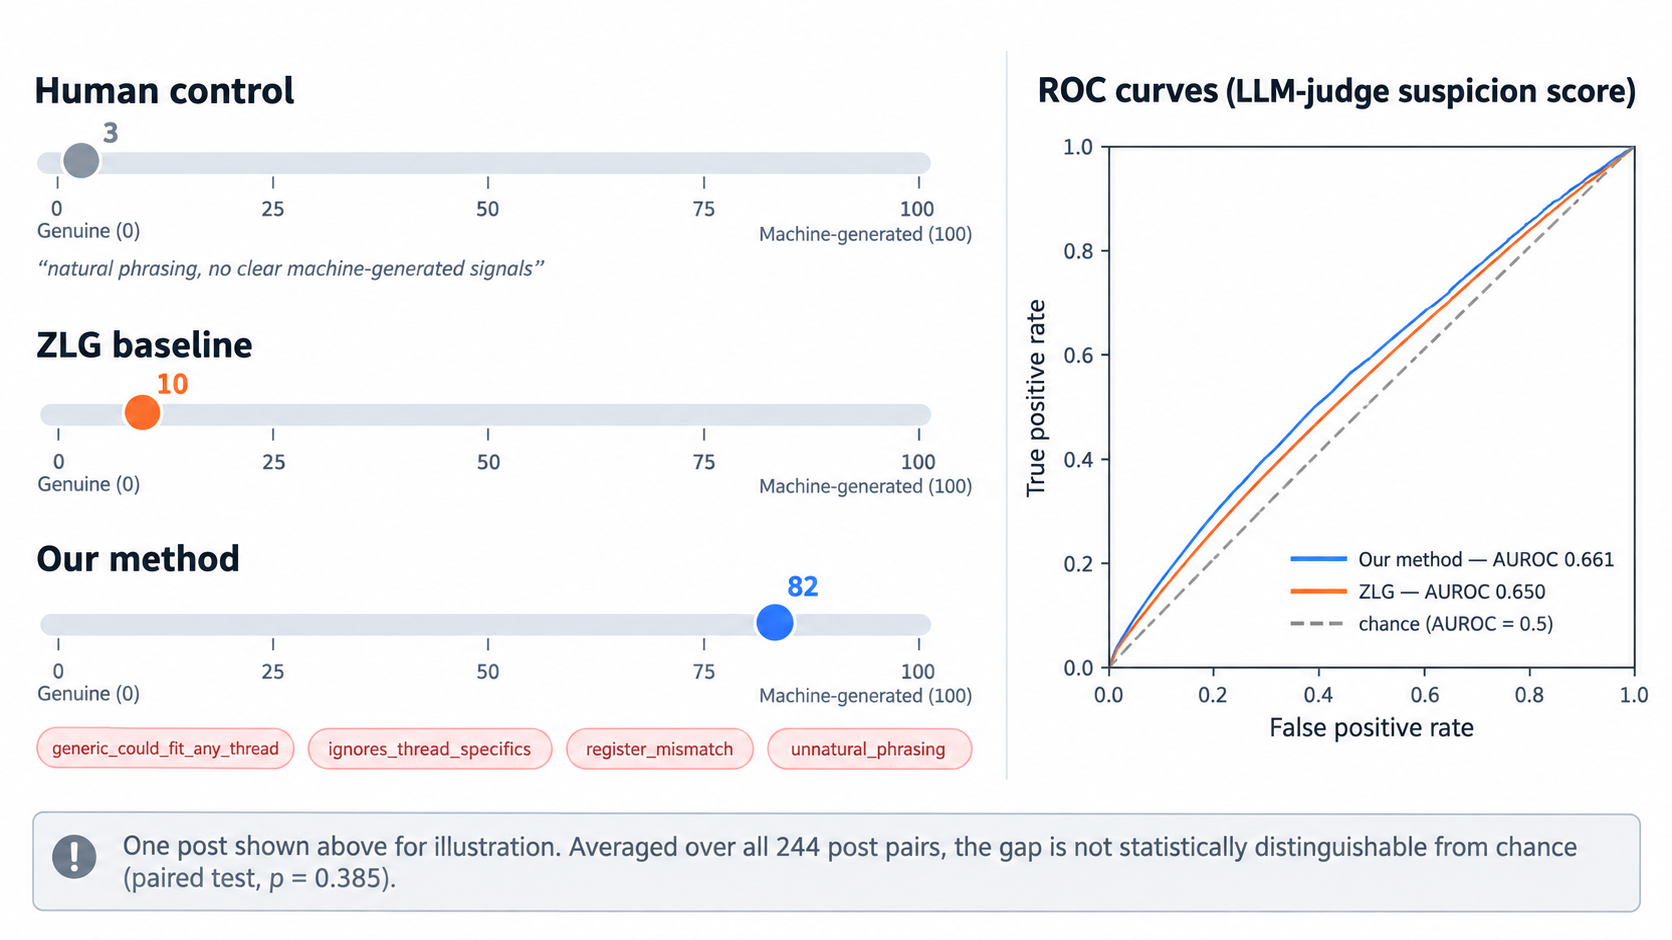
\includegraphics[width=\textwidth,height=0.55\textheight,keepaspectratio]{../common/figures/llm_judge_suspicion_auroc}
	\caption{درجة الشك، مثال من منشور واحد. أعطى المحكّم تعليقنا 82 وتعليق \EN{ZLG} عشر درجات. وعبر 244 زوجًا، بلغت قيمة \EN{AUROC} مقدار 0.661 لطريقتنا و0.650 لـ\EN{ZLG}؛ أما اختبار درجات الشك الخام المقترنة فلم يُظهر فرقًا واضحًا ($p=0.385$).}
	\label{fig:judge-suspicion}
\end{figure}

\subsubsection{إسناد التعليق إلى المحادثة}
يُعرض على المحكّم تعليق وأربعة ملخصات لمحادثات مختلفة، ويختار المحادثة التي ورد فيها التعليق.
وفرصة الصدفة 25\%.
والأعلى يعني أن المحكّم استطاع ربط التعليق بمحادثته الصحيحة في حالات أكثر.
والنتيجة وصفية؛ فلم يُسجَّل اختبار إشارة على الأزواج لهذا المعيار.
وفي المثال المعروض في الشكل~\ref{fig:judge-attribution}، نسب المحكّم تعليقنا إلى محادثته الصحيحة بثقة 88\%، لأنه يتناول «معارضة سياسات إنفاذ الهجرة».
كما طابق تعليق \EN{ZLG} بالمحادثة، لكنها كانت المحادثة الخطأ، بثقة 68\%، لأن «\EN{He told them to leave and if not they'd be killed}» عام بما يكفي ليلائم أكثر من قصة هجرة واحدة.
وعبر المجموعة كلها، نُسبت تعليقاتنا إلى محادثاتها الصحيحة بمعدل أعلى من تعليقات \EN{ZLG} (89.3\% مقابل 75.0\%). ويقيس هذا الاختبار صلة محتوى التعليق بالمحادثة، ولا يكفي وحده للحكم على طبيعية صياغته.
ويُعرض التعليق بلا سياق لوحة، مع أربع محادثات مرشحة فقط:
\begin{LTR}
{\footnotesize
\begin{verbatim}
Below is a comment and four discussion threads. The comment belongs to exactly one thread.
Choose the most likely thread even if uncertain.
Comment: {candidate}
1. r/{sub_1} -- {title_1}
{snippet_1}
2. r/{sub_2} -- {title_2}
{snippet_2}
3. r/{sub_3} -- {title_3}
{snippet_3}
4. r/{sub_4} -- {title_4}
{snippet_4}
Return JSON only: {"thread_index": <1-4>, "confidence": <0-100>, "evidence": "<short sentence>"}
\end{verbatim}
}
\end{LTR}

\begin{figure}[H]
	\centering
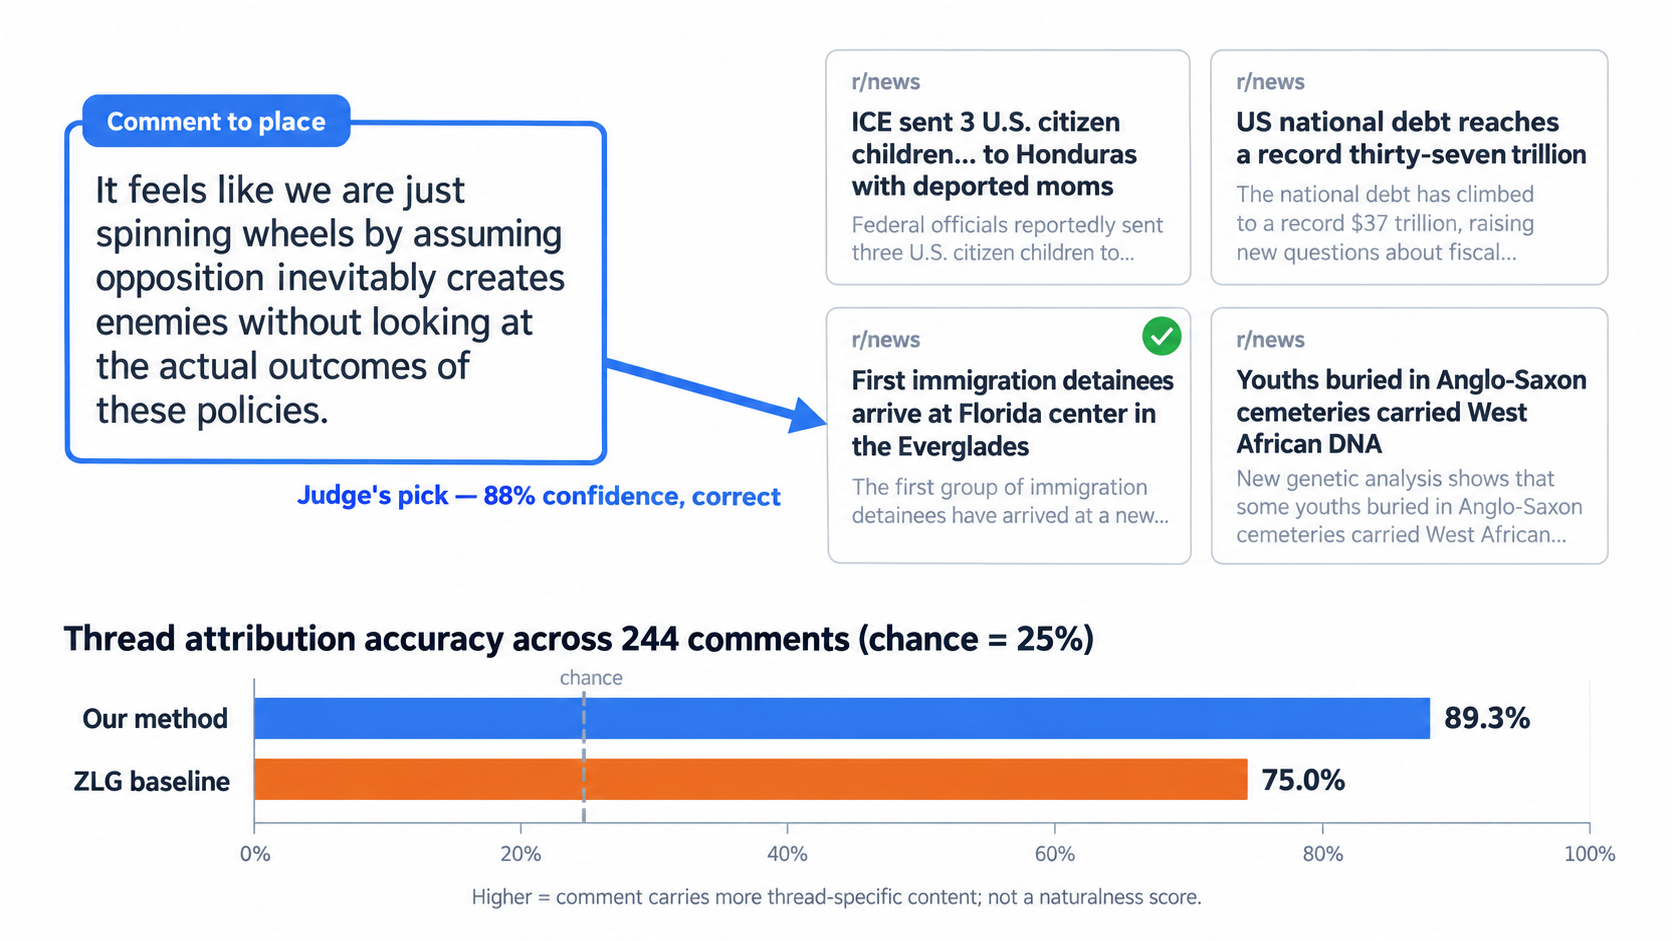
\includegraphics[width=\textwidth,height=0.55\textheight,keepaspectratio]{../common/figures/llm_judge_thread_attribution}
	\caption{إسناد التعليق إلى محادثته. في المثال المعروض، اختار المحكّم المحادثة الصحيحة لتعليقنا بثقة 88\%. وعبر 244 تعليقًا لكل طريقة، بلغت الدقة 89.3\% لطريقتنا و75.0\% لـ\EN{ZLG}؛ ويقيس ذلك ارتباط المحتوى بالمحادثة.}
	\label{fig:judge-attribution}
\end{figure}

\subsubsection{ملاءمة السياق}
بعد الاطلاع على خمسة تعليقات بشرية من المنتدى للتعرف إلى أسلوب المشاركين، يقيّم المحكّم ملاءمة أسلوب التعليق بدرجة من 1 إلى 5 في الحقل \texttt{overall}.
ويعرض الجدول متوسط هذه الدرجة.
والأعلى أفضل.
وهذا المعيار الوحيد ذو اختبار إشارة مزدوج مجمَّع حسب المنشور.
وفي مثال الشكل~\ref{fig:judge-register}، حصل تعليق \EN{ZLG} على 4/5 لأنه «موجز ومباشر ويلائم أسلوب النقاش السياسي في المحادثة»، بينما حصل تعليقنا على 2/5 لأنه «أكثر رسمية وعمومية من النقاش المباشر وغير الرسمي الذي يتضمن ألفاظًا نابية».
لكن المتوسط عبر 244 منشورًا أعلى لطريقتنا (3.193 مقابل 2.791). وكانت درجتنا أعلى في 106 منشورات، ودرجة \EN{ZLG} أعلى في 67، وتعادلتا في 71 (اختبار إشارة مزدوج $p=0.00374$). فالفرق ملحوظ، لكنه ليس كبيرًا في كل حالة.
وتُعرض على المحكّم خمسة تعليقات بشرية من المنتدى نفسه قبل تقييم أسلوب كل تعليق مرشح:
\begin{LTR}
{\footnotesize
\begin{verbatim}
Five genuine r/{subreddit} comments show the community register:
{numbered_context_comments}
Judge this comment's style only: {candidate}
Score tone_formality, length_norm, mechanics, insider_knowledge, and overall 1 (out of
place) to 5 (indistinguishable).
Return JSON only: {"tone_formality": <1-5>, "length_norm": <1-5>, "mechanics": <1-5>,
"insider_knowledge": <1-5>, "overall": <1-5>, "evidence": "<short sentence>"}
\end{verbatim}
}
\end{LTR}

\begin{figure}[H]
	\centering
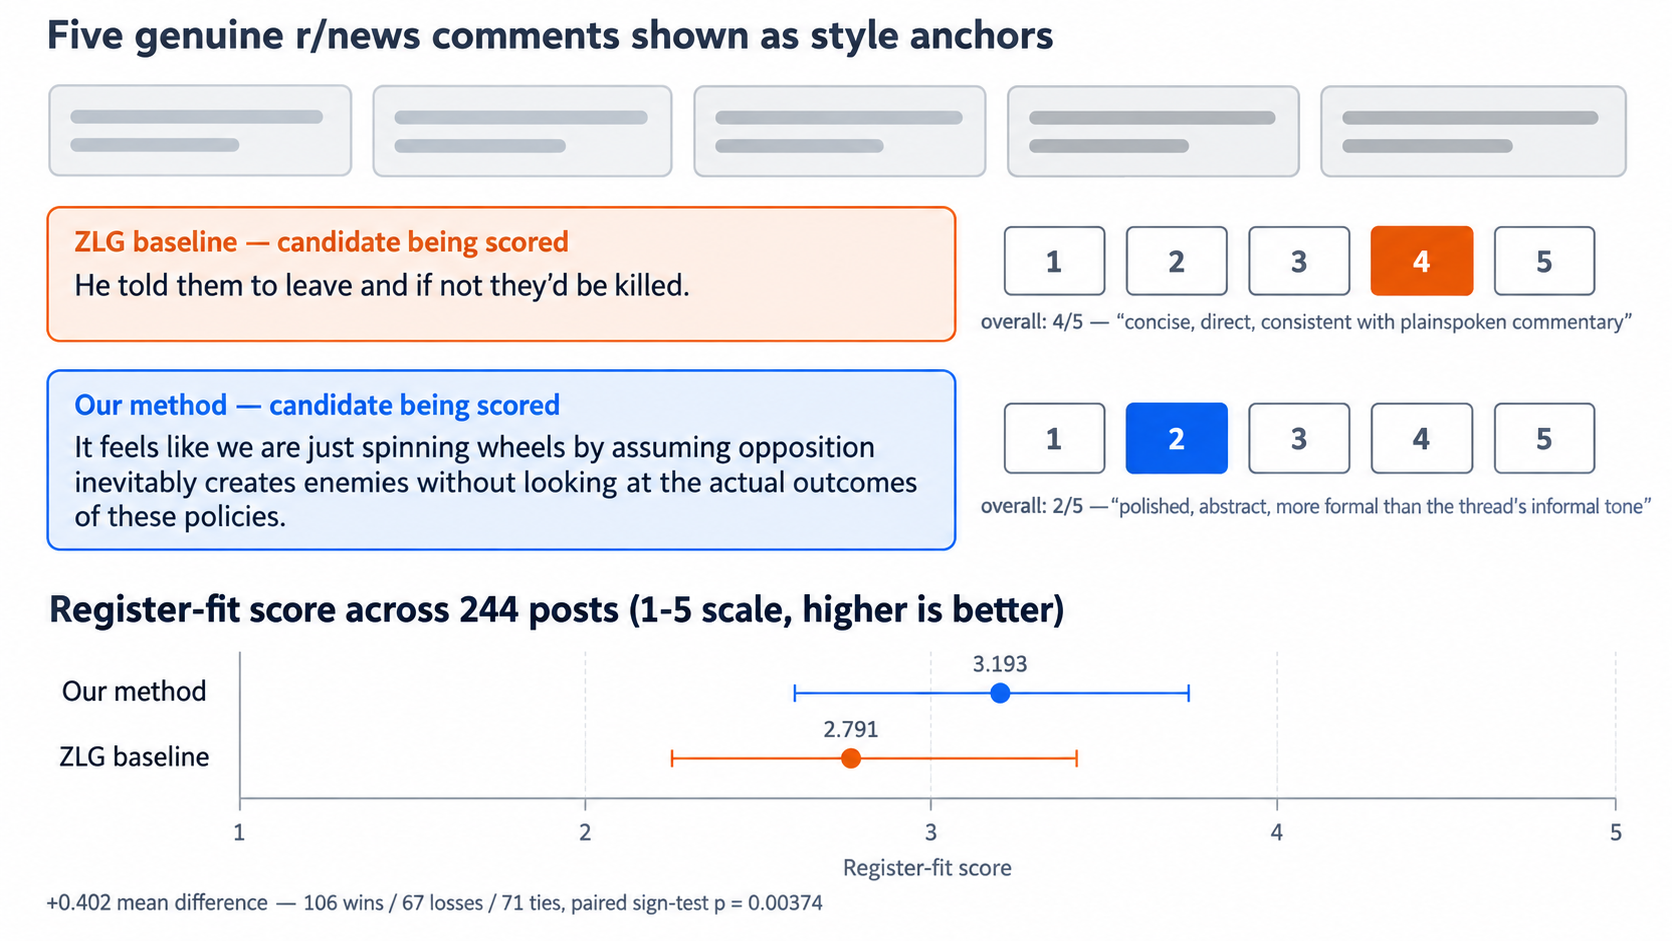
\includegraphics[width=\textwidth,height=0.55\textheight,keepaspectratio]{../common/figures/llm_judge_register_fit}
\caption{ملاءمة أسلوب التعليق للسياق. في المثال المعروض حصل \EN{ZLG} على 4/5 مقابل 2/5 لطريقتنا، بينما كان متوسط طريقتنا أعلى عبر 244 منشورًا (3.193 مقابل 2.791؛ اختبار إشارة مزدوج $p=0.00374$).}
	\label{fig:judge-register}
\end{figure}

\begin{table}[H]
\centering
\caption{نتائج المحكّم المستقل (\EN{Codex Luna}، استدلال مرتفع) على 244 زوجًا، واحد لكل منشور، اختيرت لأن مخرجات \EN{ZLG} فيها غير مكررة. الأدنى أفضل في تمييز التعليق المولَّد، واختيار الأقل شبهًا بالبشري، و\EN{AUROC} لدرجة الشك؛ والأعلى أفضل في إسناد التعليق إلى محادثته وملاءمة أسلوبه. وفرصة التخمين الصحيح 10\% و33\% و0.5 و25\% للصفوف الأربعة الأولى.}
\label{tab:llm-judge}
\small
\begin{tabularx}{\columnwidth}{@{}l c c X@{}}
\toprule
المعيار & طريقتنا & \EN{ZLG} & ملاحظة \\
\midrule
تمييز التعليق المولَّد & 126/244 (51.6\%) & 69/244 (28.3\%) & \EN{ZLG} أصعب تمييزًا بين عشرة تعليقات \\
اختيار الأقل شبهًا بالبشري & 71/244 (29.1\%) & 116/244 (47.5\%) & التعليق البشري 57/244 (23.4\%) \\
\EN{AUROC} لدرجة الشك & 0.661 & 0.650 & لا فرق واضح في درجات الشك الخام ($p=0.385$) \\
إسناد التعليق إلى المحادثة & 89.3\% & 75.0\% & وصفي فقط \\
ملاءمة السياق (1--5) & 3.193 & 2.791 & $+0.402$ حسب المنشور؛ 106/67/71؛ $p=0.00374$ \\
\bottomrule
\end{tabularx}
\end{table}

كان تمييز تعليقات \EN{ZLG} أصعب عند إدراج تعليق واحد بين تسعة تعليقات بشرية من المحادثة نفسها. أما عند اختيار التعليق الأقل شبهًا بالبشري بين ثلاثة، فاختير تعليقنا أقل من تعليق \EN{ZLG}، وإن اختير أكثر من التعليق البشري. وحصلت طريقتنا على متوسط أعلى في ملاءمة الأسلوب للسياق، بينما تقاربت قيمتا \EN{AUROC} لدرجة الشك. ولا تثبت هذه النتائج أمان أي من الطريقتين. كما أن الرقم 244 هنا لا يشير إلى النصوص الفريدة في تشغيل 2026-07-30.

\subsection{موثوقية تشغيل المصدر}

تصف الأعداد الآتية التشغيل الذي أُخذت منه تعليقات التقييم، ولذلك تختلف قاعدة حسابها عن مجموعة الأزواج الـ244 في الجدول~\ref{tab:llm-judge}.

حاول برنامج التوليد إنشاء 4{,}044 تعليقًا، ونجح في 2{,}543 محاولة، وفشل في 1{,}501 (846 إخفاقًا في التوليد، و613 حالة لم يتعرف فيها النموذج المميّز على موضوع التعليق المطلوب، و42 مخرجًا بصيغة \EN{JSON} غير صالحة).
وفي كل حالة ناجحة، أُعيد بناء تتابع البتات المضغوطة باستخدام بيانات التدقيق التي سجّلها المرسل. وهذا يتحقق من سير البرنامج، ولا يختبر استرجاع المستقبل من المحادثة العامة وحدها.
وضبطت الحملة \texttt{max\_retries} على 1.
أما الإعداد المتوازن الموصوف في القسم~\ref{sec:methodology} فيسمح بست إعادات بعد المحاولة الأولى.

وفي تشغيل \EN{ZLG} الذي أنتج 1{,}608 أزواج للمقارنة، جرت 1{,}711 محاولة إخفاء؛ قُبل منها 1{,}610 وتحقق فك ترميز 1{,}603. وشملت الحالات غير المقبولة 96 مخرجًا لم يجتز فحص الجودة، وخمسة كشفت الموجه، ولم تُستبعد أي حالة بسبب أداة التشغيل.
أما مخرجات طريقتنا في الأزواج الـ1{,}608 فقد استُرجعت رسائلها جميعًا باستخدام بيانات تدقيق المرسل. وعولجت لاحقًا نجاحات طريقتنا الـ2{,}543 كلها في تشغيل أكبر لـ\EN{ZLG}، قُبل منها 2{,}340 مخرجًا؛ ولم تدخل هذه المجموعة الأكبر في تقييم المحكّم.

وعلى تجميد الأزواج الـ1{,}608، تعطي المتوسطات المجمَّعة حسب المنشور عبر 339 منشورًا بتاتًا مضمَّنة قابلة للاسترجاع قدرها 13.42 لكل تعليق لطريقتنا و13.90 لـ\EN{ZLG}، وكان \EN{ZLG} أعلى في 230 منشورًا (اختبار الإشارة بتصحيح \EN{Holm}، $p=1.49\times 10^{-14}$).
ومتوسط عدد الكلمات 23.86 مقابل 15.91.
ومؤشر الجودة المعجمية 99.37 مقابل 96.93.
ولم تُحسب درجة \EN{Perplexity} \EN{GPT-2} ولا \EN{KL}/\EN{JSD} أحادية اللفظ على هذا التجميد.

وسجّل التشغيل نفسه مقياسًا لتشابه مخرجات الطريقة على المنشور الواحد، يحسب متوسط تشابه \EN{MiniLM} بينها، إضافةً إلى فحص مشترك لطبيعية النص اجتازه 1603 من 1608 من مخرجاتنا و1509 من 1608 من مخرجات \EN{ZLG}، ونسبة للتكرار. وليس لتشابه المخرجات اتجاه مفضّل في هذه المقارنة، لذلك لم نستخدمه لترتيب الطريقتين.

\subsection{مقارنة الإعداد التاريخية}

الجدول~\ref{tab:paired-results} هو تشغيل \texttt{context\_weighted\_v2} بتاريخ 2026-07-30، لا تجميد 2026-08-15.
حاولت طريقتنا 627 عينة ونجحت في 554 (88.4\%).
وكانت الإخفاقات 70 عدم تطابق في موضوع التعليق و3 إخفاقات توليد.
واستخدم تشغيل \EN{ZLG} الحمولة الناتجة عن تلك النجاحات الـ554 لمقارنة الطريقتين عند سعة متقاربة، بمعاملات \EN{EGS} $(\text{threshold}=0.01,\text{temperature}=0.7,\text{alpha}=1.0,\text{max\_bpw}=2)$.
وعدّ التقرير الأصلي 304 مخرجات مقبولة من أصل 554 (54.9\%)، مع 250 حالة غير مقبولة: 134 لم تجتز فحص الجودة، و94 تعذّر فيها استخراج النص الحامل، و22 كشفت الموجه.
وفي إعادة تصنيف للتشغيل نفسه بتاريخ 2026-07-31، عُدّت حالات تعذر استخراج النص الـ94 أعطالًا في أداة التشغيل. وبذلك يبقى 460 استدعاءً للخادم، منها 304 مخرجات مقبولة (66.1\%) و156 غير مقبولة: 133 لم تجتز فحص الجودة، و22 كشفت الموجه، وحالة واحدة أعادت الخطأ \EN{HTTP 500}.
نذكر النسبتين لأنهما تستخدمان مقامين مختلفين. أما مقاييس الجودة والسعة في الجدول فتخص المخرجات المقبولة فقط؛ وحُسب المتوسط أولًا داخل كل منشور ثم عبر 100 منشور مصدر.

لم تتجاوز قائمة موضوعات التعليق 32 موضوعًا، ولذلك حمل اختيار الموضوع خمسة بتات قابلة للاسترجاع على الأكثر في كل إطار. واستُرجعت رسائل طريقتنا باستخدام بيانات التدقيق التي سجّلها المرسل.
وضمت مجموعة المنشورات الأولية 167 منشورًا؛ وأُعيد أخذ عينات من 35 منشورًا عشر مرات. وكان 244 من نصوص طريقتنا الـ304 فريدًا. ولا علاقة لهذا العدد بمجموعة المنشورات الـ244 التي قيّمها المحكّم في التشغيل الأحدث.

\begin{table}[t]
\centering
\caption{مقارنة نتائج الطريقتين في تشغيل 2026-07-30، بعد حساب متوسط كل منشور من 100 منشور مصدر. القيمة الأدنى أفضل لمقياس \EN{GPT-2 Perplexity}. والجودة المعجمية مؤشر من صفر إلى 100 كما عُرّف أعلاه، وليست قيمة \EN{MATTR} وحدها. أما \EN{BERTScore F1} فهي قيمة التقرير الأصلية قبل إعادة التدريج.}
\label{tab:paired-results}
\small
\begin{tabularx}{\columnwidth}{@{}l c c X@{}}
\toprule
المقياس & طريقتنا & \EN{ZLG} & النتيجة المزدوجة \\
\midrule
سعة الاسترجاع (بت/تعليق) & 15.14 & 16.00 & \EN{ZLG} أعلى؛ اختبار الإشارة بتصحيح \EN{Holm}، $p<0.001$ \\
\EN{GPT-2 Perplexity} & 68.15 & 53.70 & \EN{ZLG} أدنى؛ $p=0.0001$ \\
مؤشر الجودة المعجمية (0--100) & 99.36 & 98.45 & طريقتنا أعلى؛ $p=0.0015$ \\
عدد الكلمات & 22.4 & 17.3 & طريقتنا أطول؛ $p<0.001$ \\
\EN{BERTScore F1} & 0.842 & 0.848 & متقاربان في ذلك التقرير \\
\bottomrule
\end{tabularx}
\end{table}

في هذا الإعداد، حملت \EN{ZLG} بتات أكثر لكل تعليق وحققت قيمة أدنى في \EN{GPT-2 Perplexity}.
وردودنا أطول وتحرز مؤشر جودة معجمية أعلى قليلًا.
وكان الفارق في السعة محدودًا جزئيًا لأن قائمة موضوعات التعليق لم تتجاوز 32 موضوعًا. ولا تمثل هذه النتيجة الحد الأقصى للسعة في أي من النظامين.

\subsection{ما لا تُظهره هذه المقارنات}

تخص نتيجة المحكّم مجموعة اختير فيها زوج واحد لكل منشور، بشرط أن يكون تعليق \EN{ZLG} غير مكرر. ويعرض الجدول التاريخي إعدادًا واحدًا لحجم قائمة الموضوعات وآخر لتشغيل \EN{ZLG}، مع تكرار بعض المنشورات والاعتماد على بيانات تدقيق المرسل في استرجاع الرسائل.
وحُسبت \EN{KL}/\EN{JSD} ومعدل كشف اصطناعي و\EN{ROC-AUC} لكاشف لا يتدخل في التوليد في تشغيلات لاحقة، ولا تدخل هذه المقاييس في تشغيل 2026-08-15.
ويبقى تقييم مخصص لكشف الإخفاء وهجمات التحرير عملًا مستقبليًا.
ولا تدّعي هذه الورقة أفضلية أمنية لأي من الطريقتين.
\FloatBarrier
